\newpage
\section{Prospetto economico}
In questo paragrafo sono presentate, per ciascun periodo del progetto, le ore di impegno calcolate a preventivo per i ruoli coinvolti, divise tra ore di lavoro e ore contabilizzate.\\
 Si ricorda che il periodo di \ARM\ non è a carico del \termine{committente} e quindi non sarà considerata nel calcolo del preventivo.
 
\subsection{\ARD}
Nel periodo riguardante la fase di \ARD\ le ore tra i ruoli sono state divise nel seguente modo:

\begin{table}[h]
	\begin{center}
		\begin{tabular}{|l|c|c|}
			\hline
			\textbf{Ruolo}	& \textbf{Ore} & \textbf{Costo} \\
			\hline
			\textit{\Pm} &	3	&	90\\
			\hline
			\textit{\Am}	&	3	&	 60	\\
			\hline
			\textit{\An}	&	30	&	 750	\\
			\hline
			\textit{\Ver}	 & 14	&	 210	\\
			\hline
			\textbf{Totale} &	 \textbf{50}	&	\textbf{1110}\\
			\hline
		\end{tabular}
	\end{center}
	\caption{Incidenza ore su costo per ruolo, \ARD}
\end{table}

\begin{figure}[H]
	\centering 
	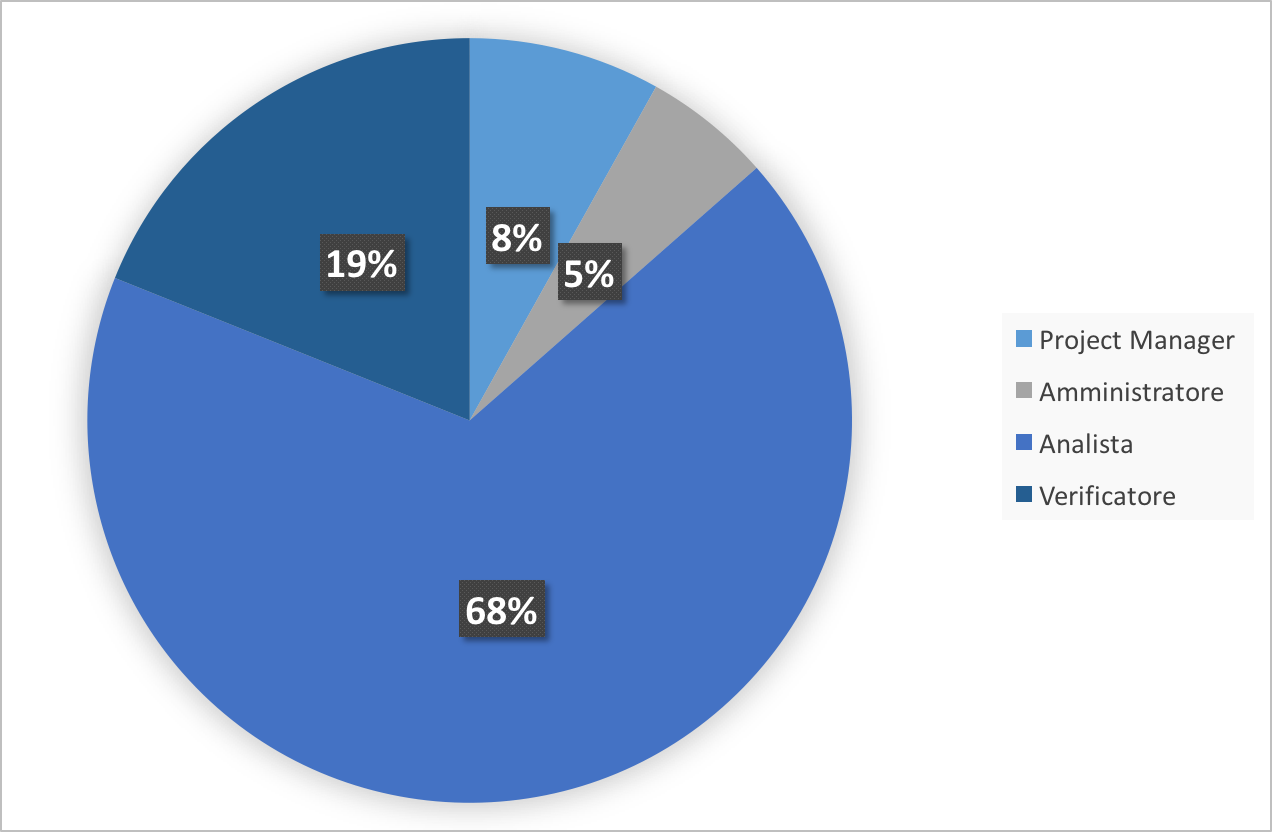
\includegraphics[scale=0.7]{Immagini/GraficiTorteSezione6/ARD.png}
	\caption{Costo per ruolo, \ARD}
\end{figure}

\newpage
\subsection{\PA}
Nel periodo riguardante la \PA\ le ore tra i ruoli sono state divise nel seguente modo:

\begin{table}[h]
	\begin{center}
		\begin{tabular}{|l|c|c|}
			\hline
			\textbf{Ruolo}	& \textbf{Ore} &	\textbf{Costo}	 \\
			\hline
			\textit{\Pm}	&	6	&	180\\
			\hline
			\textit{\Am}	&	7	&	140\\
			\hline
			\textit{\Prog}	&	120	&	2640\\
			\hline
			\textit{\Ver}	&	65	&	975\\
			\hline
			\textbf{Totale}	&	\textbf{198}	&	\textbf{3935}\\
			\hline
		\end{tabular}
	\end{center}
	\caption{Incidenza ore su costo per ruolo, \PA}
\end{table}

\begin{figure}[H]
	\centering 
	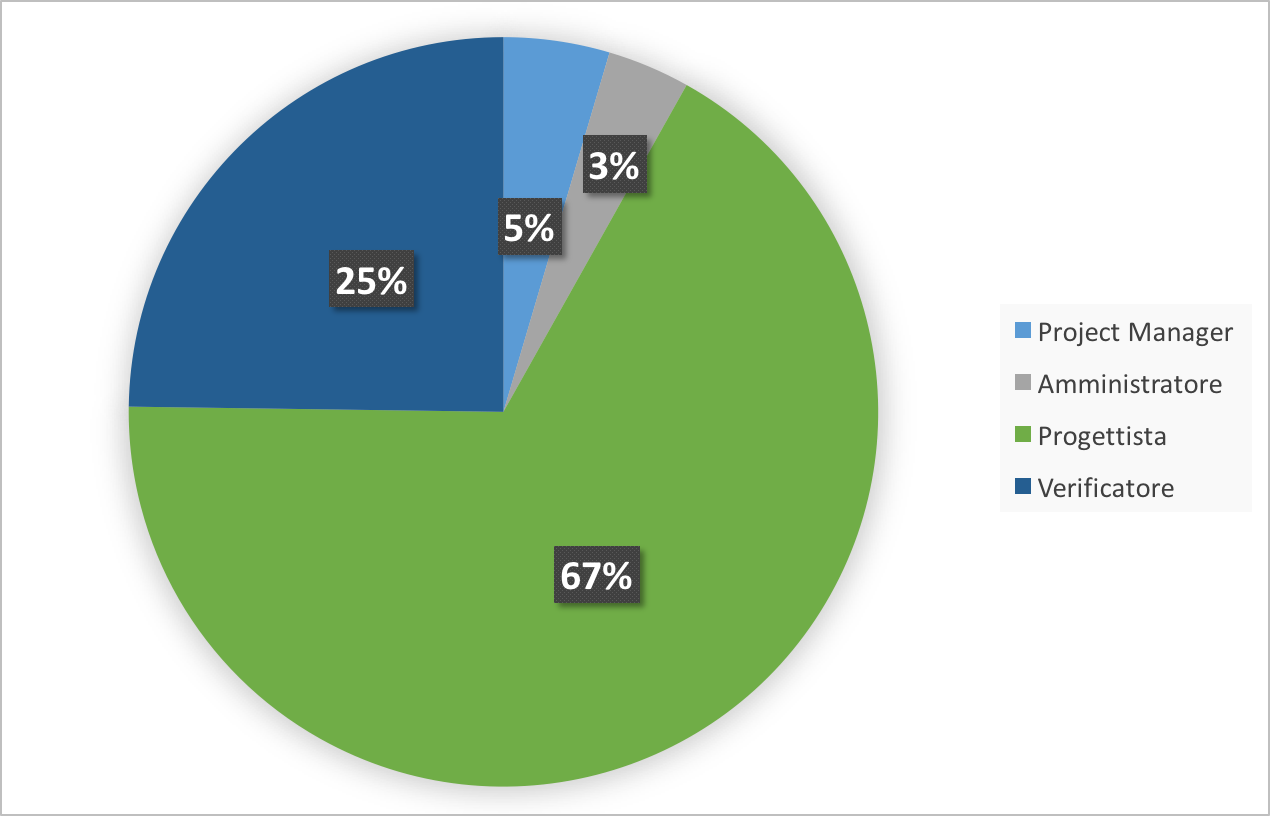
\includegraphics[scale=0.7]{Immagini/GraficiTorteSezione6/PA.png}
	\caption{Costo per ruolo, \PA}
\end{figure}

\newpage
\subsection{\PD\ e \COD}
Nel periodo riguardante la \PD\ e \COD\ le ore tra i ruoli sono state divise nel seguente modo:
\begin{table}[h]
	\begin{center}
		\begin{tabular}{|l|c|c|}
			\hline
			\textbf{Ruolo}	& \textbf{Ore} &	\textbf{Costo}	 \\
			\hline
			\Pm &	20 & 600\\
			\hline
			\Am	&	12 & 240\\
			\hline
			\Prog	&	107 & 2354\\
			\hline
			\Progr	&	200 & 2160\\
			\hline
			\Ver	&	139 & 1875\\
			\hline
			\textbf{Totale} &	 \textbf{478}	&	\textbf{7229}\\
			\hline
		\end{tabular}
	\end{center}
	\caption{Incidenza ore su costo per ruolo, \PD\ e \COD}
\end{table}

\begin{figure}[H]
	\centering 
	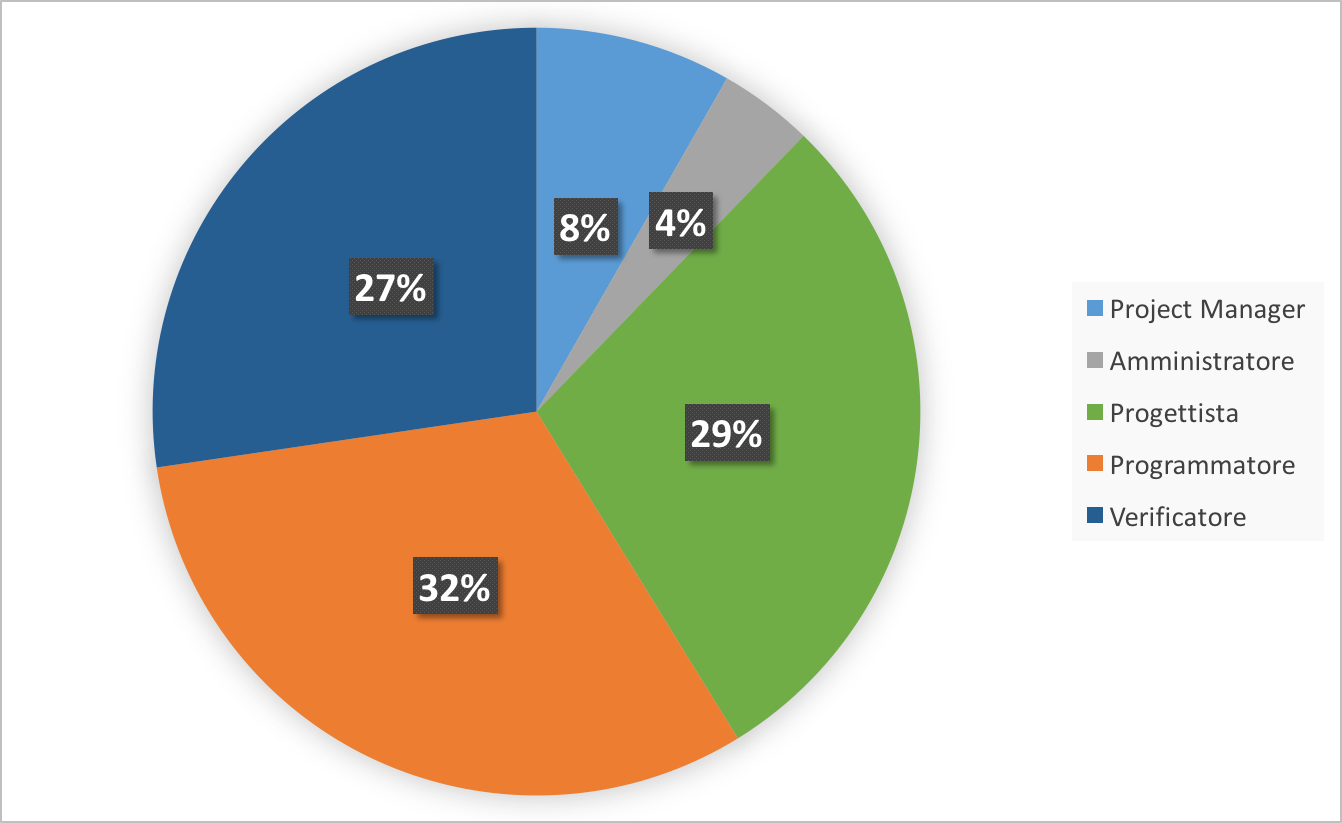
\includegraphics[scale=0.7]{Immagini/GraficiTorteSezione6/PDCOD.png}
	\caption{Ore per ruolo, \PD\ e \COD}
\end{figure}

\newpage
Fino alla \RP\ sono state pianificate 121 delle ore descritte in precedenza suddivise come segue:
\begin{table}[h]
	\begin{center}
		\begin{tabular}{|l|c|c|}
			\hline
			\textbf{Ruolo}	& \textbf{Ore} &	\textbf{Costo}	\\
			\hline
			\Pm &	7 & 210\\
			\hline
			\Am	&	7 & 140\\
			\hline
			\Prog	&	65 & 1430\\
			\hline
			\Ver	&	42 & 630\\
			\hline
			\textbf{Totale} &	 \textbf{121}	&	\textbf{2410}\\
			\hline
		\end{tabular}
	\end{center}
	\caption{Incidenza ore su costo per ruolo, \PD\ e \COD\ fino a \RP}
\end{table}

\begin{figure}[H]
	\centering 
	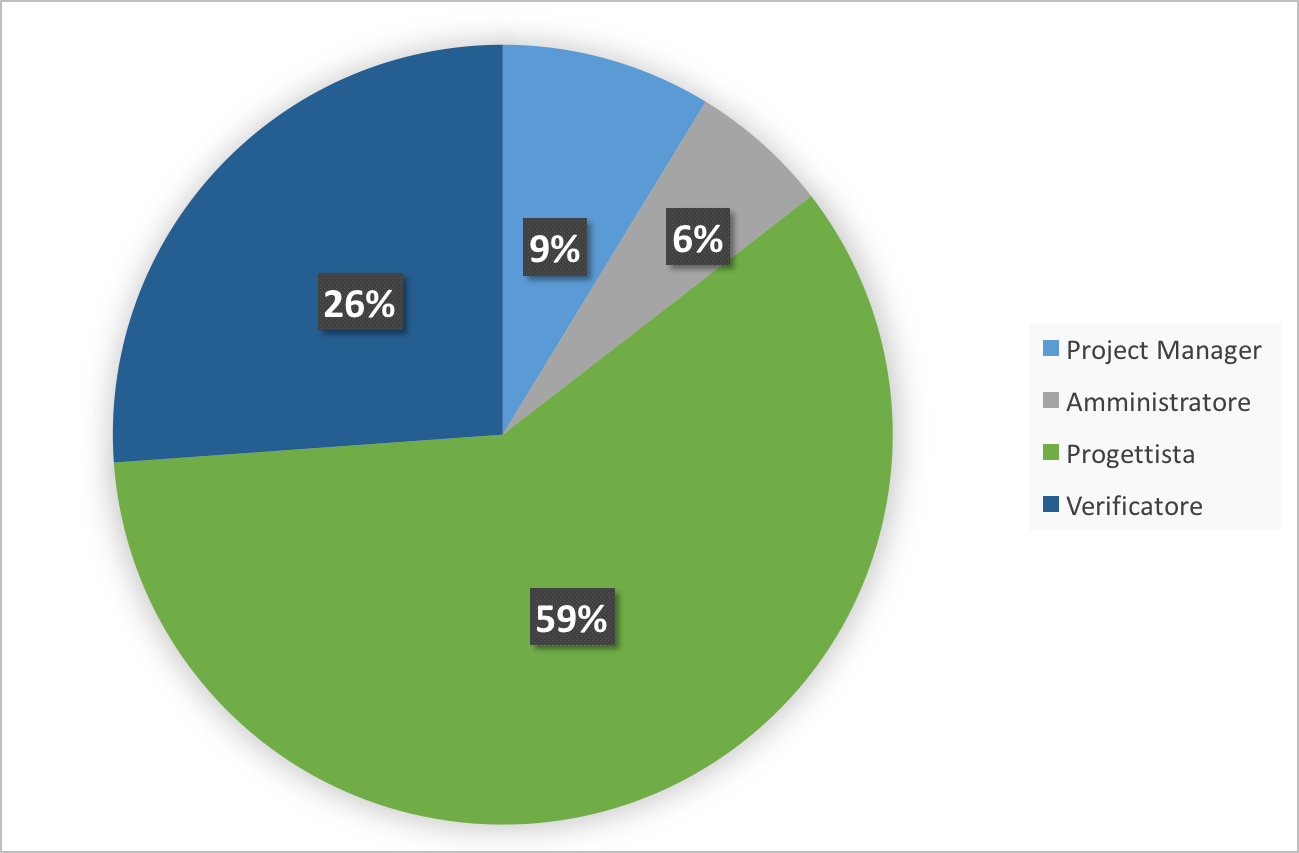
\includegraphics[scale=0.7]{Immagini/GraficiTorteSezione6/PD.png}
	\caption{Ore per ruolo, \PD\ e \COD\ fino a \RP}
\end{figure}

\newpage
Mentre dalla \RP\ fino al termine coincidente con la consegna per la \RQ\ le 357 ore rimanenti sono suddivise come segue:

\begin{table}[h]
	\begin{center}
		\begin{tabular}{|l|c|c|}
			\hline
			\textbf{Ruolo}	& \textbf{Ore} &	\textbf{Costo}	\\
			\hline
			\Pm &	13 & 390\\
			\hline
			\Am	&	5 & 100\\
			\hline
			\Prog	&	42 & 924\\
			\hline
			\Progr	&	200 & 2160\\
			\hline
			\Ver	&	97 & 1245\\
			\hline
			\textbf{Totale} &	 \textbf{357}	&	\textbf{4819}\\
			\hline
		\end{tabular}
	\end{center}
	\caption{Incidenza ore su costo per ruolo, \PD\ e \COD\ da \RP\ fino a \RQ}
\end{table}

\begin{figure}[H]
	\centering 
	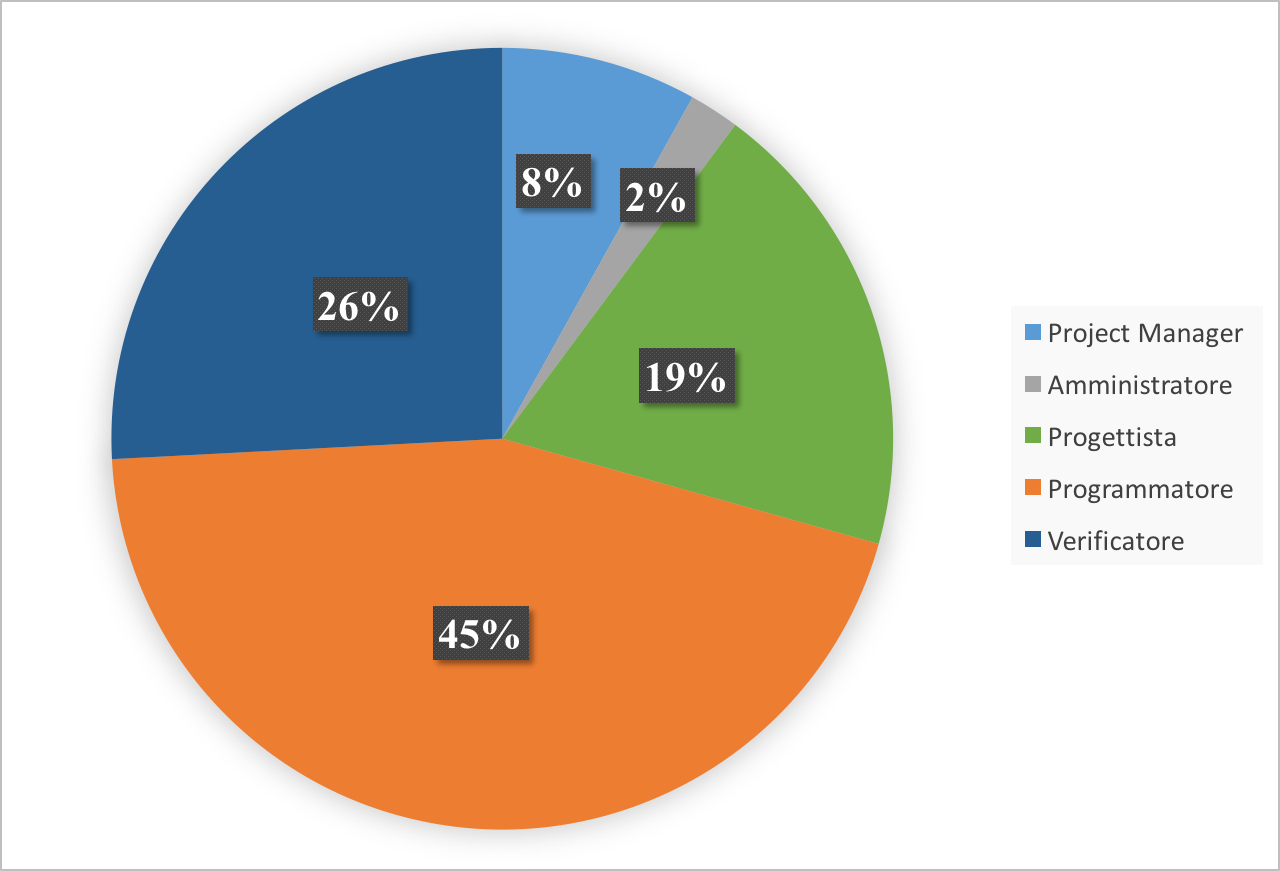
\includegraphics[scale=0.7]{Immagini/GraficiTorteSezione6/COD.png}
	\caption{Ore per ruolo, \PD\ e \COD\ da \RP\ fino a \RQ}
\end{figure}

\newpage
\subsection{\VV}
Nel periodo riguardante la \VV\ le ore tra i ruoli sono state divise nel seguente modo:

\begin{table}[h]
	\begin{center}
		\begin{tabular}{|l|c|c|}
			\hline
			\textbf{Ruolo}	& \textbf{Ore} &	\textbf{Costo}	 \\
			\hline
			\textit{\Pm}	&	8	&	240		\\
			\hline
			\textit{\Am}	&	3	&	60		\\
			\hline
			\textit{\Prog}	&	6	&	132	\\
			\hline
			\textit{\Progr}	&	8	&	120	\\
			\hline
			\textit{\Ver}	&	53	&	795	\\
			\hline
			\textbf{Totale}	&	\textbf{78}	&	\textbf{1347}	\\
			\hline
		\end{tabular}
	\end{center}
	\caption{Incidenza ore su costo per ruolo, \VV}
\end{table}

\begin{figure}[H]
	\centering 
	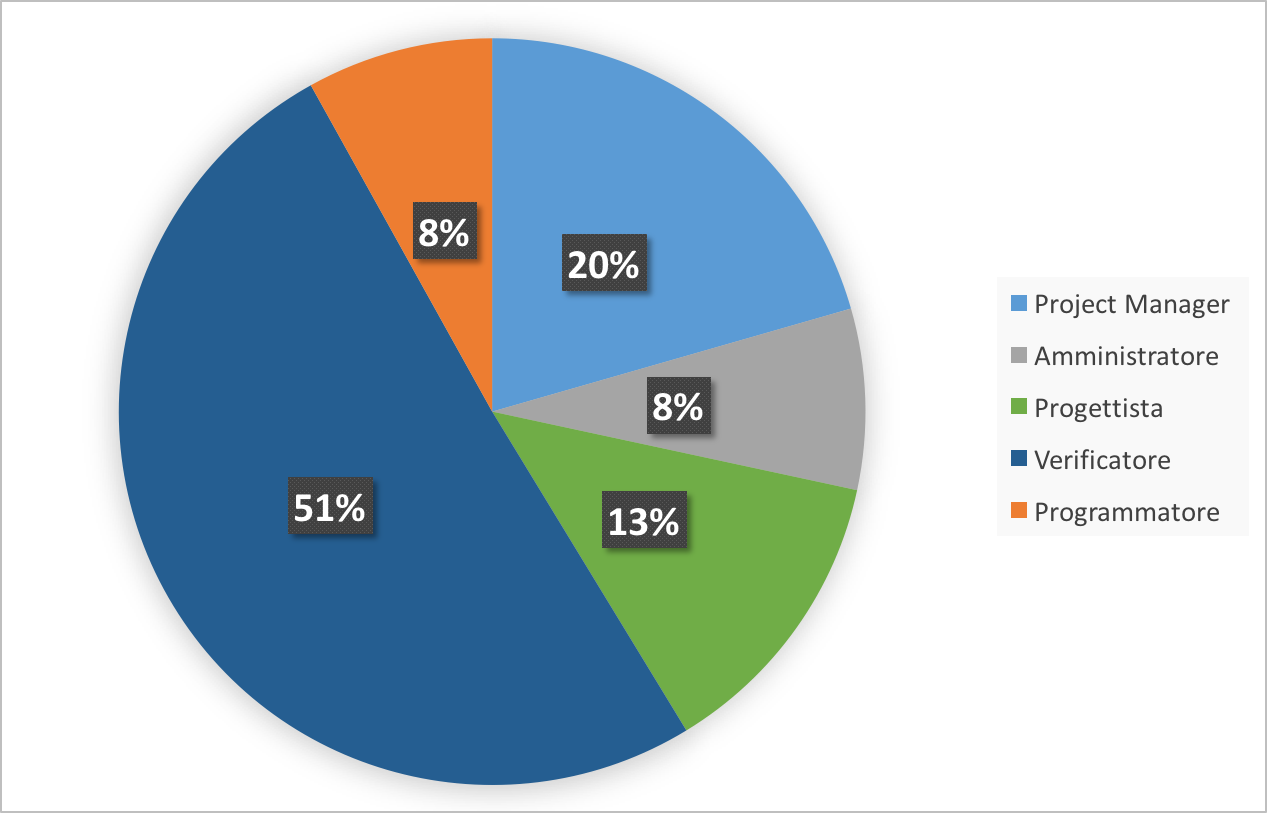
\includegraphics[scale=0.7]{Immagini/GraficiTorteSezione6/VV.png}
	\caption{Costo per ruolo, \VV}
\end{figure}

\newpage
\subsection{Totale}
\subsubsection{Ore totali}
Le ore totali, previste per la realizzazione dell'intero progetto, comprese le ore di investimento e autoapprendimento, sono riportate nella tabella seguente.

\begin{table}[h]
	\begin{center}
		\begin{tabular}{|l|c|c|c|}
			\hline
			\textbf{Ruolo}	& \textbf{Ore} &	\textbf{Ore remunerabili}	 &\textbf{Costo} \\
			\hline
			\textit{\Pm}	&	57	&	37	&	1110	\\
			\hline
			\textit{\Am}	&	44	&	25	&	500	\\
			\hline
			\textit{\An}	&	105	&	30	&	750	\\
			\hline
			\textit{\Prog}	&	233	&	233	&	5126	\\
			\hline
			\textit{\Progr}	&	208	&	152	&	2280	\\
			\hline
			\textit{\Ver}	&	336	&	257	&	3855	\\
			\hline
			\textbf{Totale}	&	\textbf{983} & \textbf{734} & \textbf{13621}	\\
			\hline
		\end{tabular}
	\end{center}
	\caption{Costo totale per ruolo}
\end{table}

\begin{figure}[H]
	\centering 
	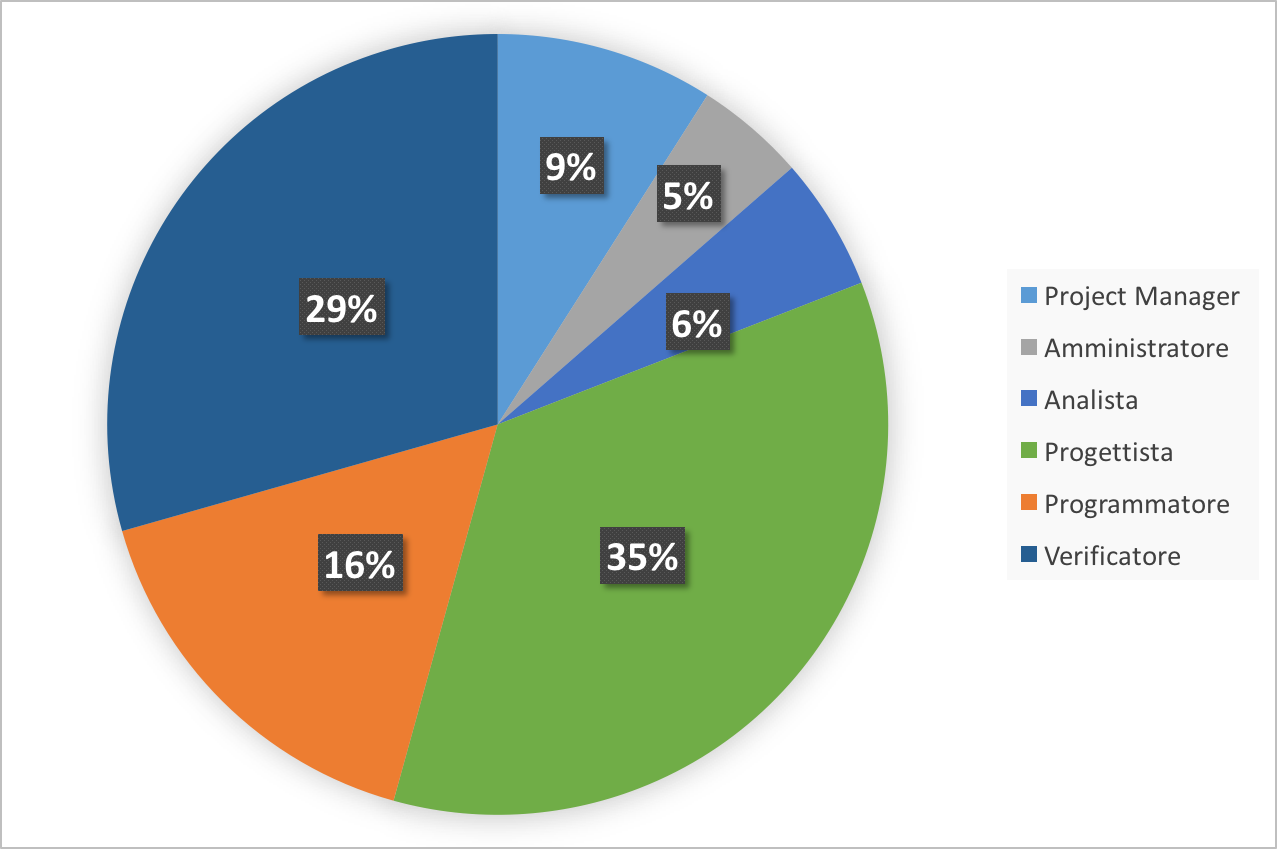
\includegraphics[scale=0.7]{Immagini/GraficiTorteSezione6/TOT.png}
	\caption{Costo totale per ruolo}
\end{figure}

\subsubsection{Conclusioni}
Il costo totale del progetto, indicato nella tabella 20, ammonta a \textbf{\euro 13621} rispettando il primo impegno preso al momento della gara per aggiudicarsi il capitolato.\\